\subsection{Чтение исходных данных}

Для начала, прочитаем \texttt{.wav} файл в виде массива точек и выведем его график (см. рисунок \ref{fig:source_wavwform}).

\begin{figure}
    \centering
    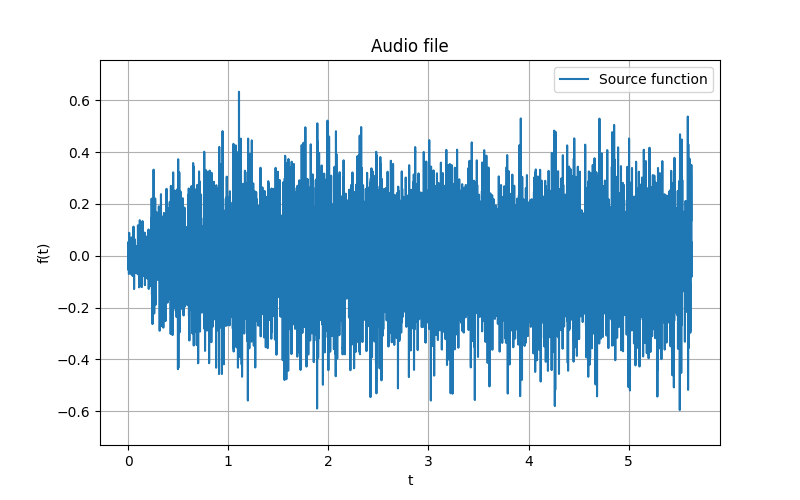
\includegraphics[width=\textwidth]{../results/Source waveform.png}
    \caption{График исходного \texttt{.wav} файла}
    \label{fig:source_wavwform}
\end{figure}

\subsection{Нахождение образа исходного сигнала}

Образ исходного сигнала находится с помощью преобразования Фурье. Для этого используется функция \texttt{fft} из библиотеки \texttt{numpy}. После нахождения образа сигнала, мы можем построить его график (см. рисунок \ref{fig:image}).

\begin{figure}
    \centering
    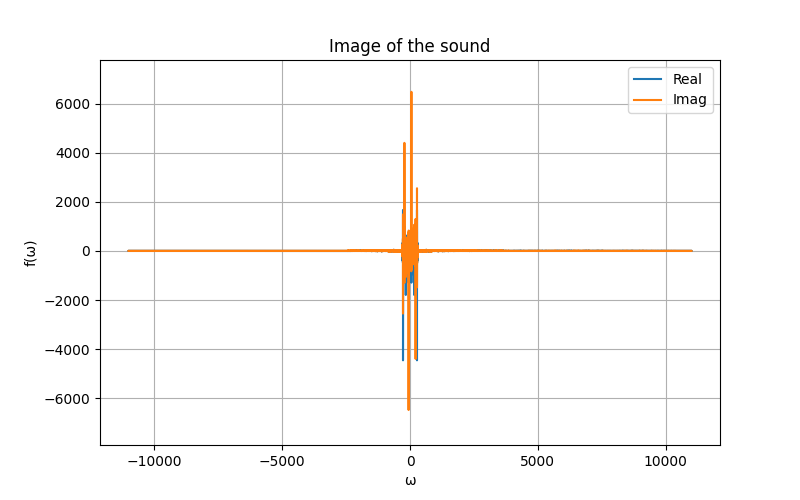
\includegraphics[width=\textwidth]{../results/image.png}
    \caption{График образа исходного сигнала}
    \label{fig:image}
\end{figure}

\FloatBarrier
\subsection{Определение частот с шумом}
Заметим, что на графике образа есть ярко выраженные пика в окрестности нуля. Остальная часть образа кажется равной нулю, но это не так, там есть малые значения, неразличимые из-за масштаба. 
Обнулим все частоты, сильно \textit{выбивающиеся} из общей картины $(\omega = \pm 300)$, и построим график (см. рисунок \ref{fig:clipped_image}).

\begin{figure}
    \centering
    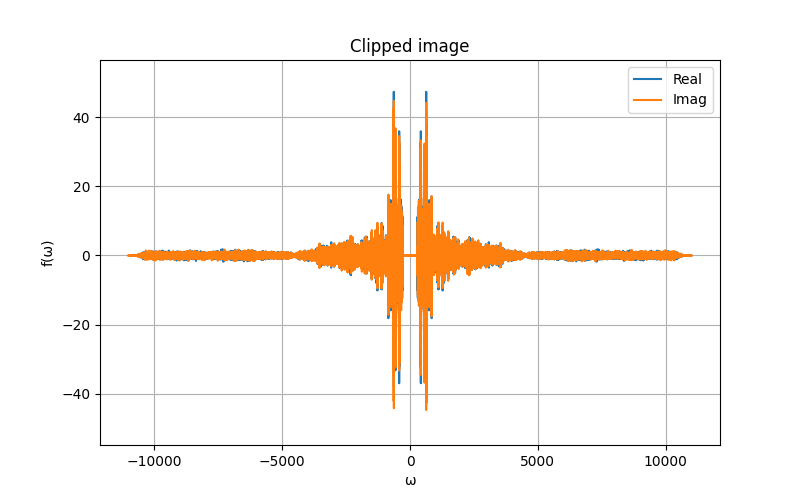
\includegraphics[width=\textwidth]{../results/Clipped image.png}
    \caption{График обрезанного образа исходного сигнала}
    \label{fig:clipped_image}
\end{figure}

Теперь стали заметны остальные значения. Максимум функции снизился $\approx 6000$ до $\approx 40$. Теперь частоты в образе распределены гораздо более равномерно, что похоже на образ аудио с голосом. 

\subsection{Обратное преобразование}

Теперь, когда мы нашли образ сигнала и обрезали его, мы можем восстановить исходный сигнал с помощью обратного преобразования Фурье. Для этого используется функция \texttt{ifft} из библиотеки \texttt{numpy}. 
После нахождения обратного преобразования, мы можем построить его график (см. рисунок \ref{fig:restored_audio}). 
График звуковой волны стал менее равномерным, что больше похоже на запись голоса. Сохраним полученный сигнал как аудио и послушаем его. 

Запись стала чистой, все шумы ушли, при этом речь диктора не исказилась, по крайне меме, на слух. Из этого можно сделать вывод, что шумы были исключительно низкочастотными и от них удалось полностью избавиться. 

\begin{figure}
    \centering
    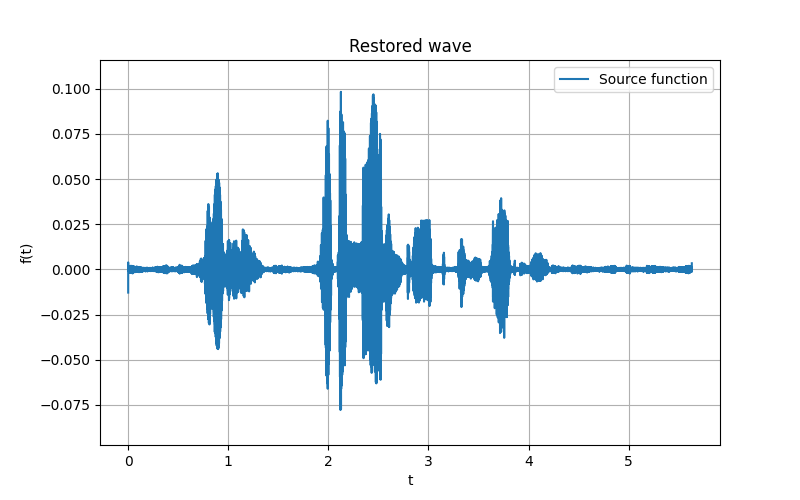
\includegraphics[width=\textwidth]{../results/Restored audio file.png}
    \caption{График фильтрованной версии исходного сигнала}
    \label{fig:restored_audio}
\end{figure}

Отфильтрованная запись доступна по \href{https://drive.google.com/file/d/1xV_qfqg4C-Z8WqTi6AU7sM3sAt7slwk1/view?usp=share_link}{ссылке}